\documentclass[a4paper]{article}
\usepackage[dutch]{babel}
\usepackage{amsmath}
\usepackage{graphicx}
\usepackage{epstopdf}

\title{Technisch Wetenschappelijke Software: Project deel 1}
\author{Dries De Samblanx}
\date{dindag 3 november 2015}

\newcommand{\opgave}[1]{\section*{Opgave #1}}
\newcommand{\dx}{\Delta x}
\newcommand{\dy}{\Delta y}
\newcommand{\dz}{\Delta z}
\newcommand{\dt}{\Delta t}

\begin{document}
\maketitle

\section*{Matrix Input/Output}

2 ontwerpbeslissingen: -type van Matrix, opslaan in transposes

De basis van het project is de invoer en uitvoer van matrices. De manier waarop we deze bijhouden in een 

\opgave{2}

De oplossing van opgave 2. Zie figuur~\ref{figuurtje}.

\begin{figure}
\begin{center}
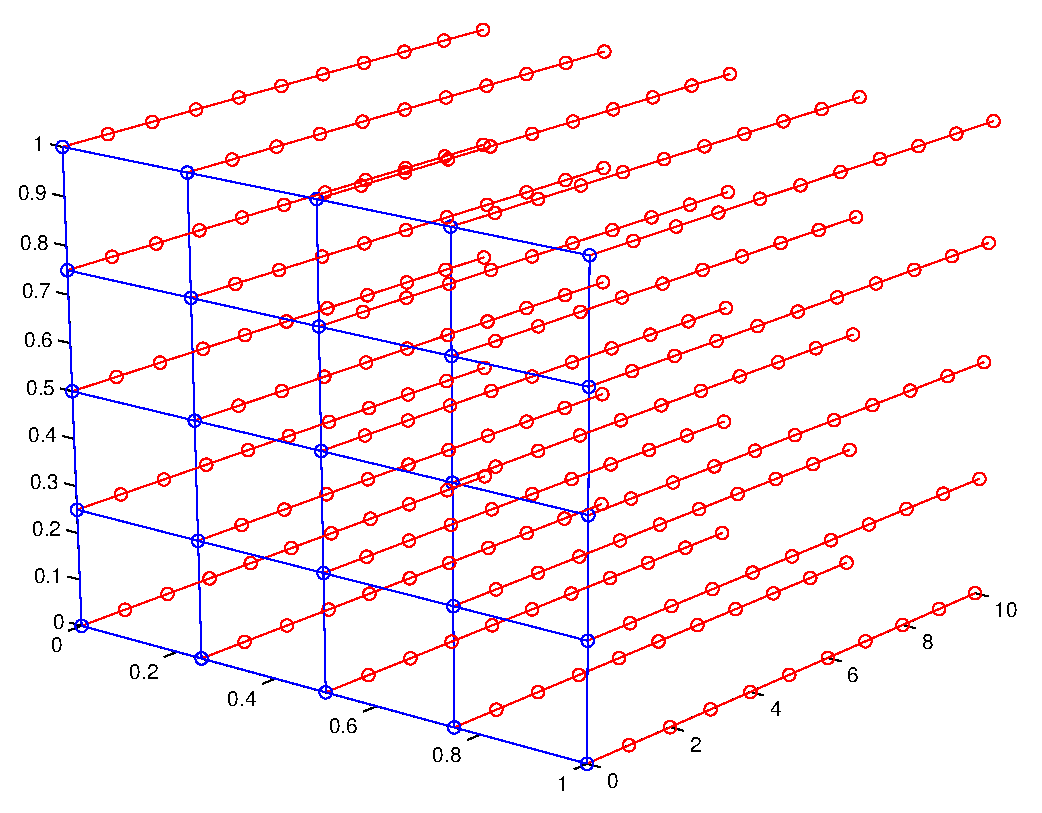
\includegraphics[width=0.4\textwidth]{figuurtje.eps}
\end{center}
\caption{Een figuurtje.}
\label{figuurtje}
\end{figure}


\opgave{3}

Zie tabel~\ref{tab1} en vergelijking~\eqref{vgl}.

\begin{table}
\begin{center}
\begin{tabular}{r|llc}
getal & cijfer & c & c \\\hline
een & 1 & 1 & 1 \\
tien & 10 & 10 & 10 \\
honderd & 100 & 100 & 100
\end{tabular}
\end{center}
\caption{Een tabel}
\label{tab1}
\end{table}

\end{document}
